%%%%%%%%%%%%%%%%%%%%%%%%%%%%%%%%%%%%%%%%%%%%%%%%%%%%%%%%%%
%%                                                      %% 
%%      Crowdmark LaTeX Exam Template v0.1              %%
%%                2013-09-20                            %%
%%                                                      %%
%%           Comments or Suggestions?                   %%
%%          email: info@crowdmark.com                   %% 
%%%%%%%%%%%%%%%%%%%%%%%%%%%%%%%%%%%%%%%%%%%%%%%%%%%%%%%%%%

\documentclass[14pt, oneside]{memoir}
\pagestyle{plain}

\usepackage{array, amssymb}
\extrarowheight=5pt
\voffset=-20pt
\textheight=9.5in
%\topmargin=2in
\usepackage{mathtools}
%\usepackage{amsthm}
\usepackage{xcolor}
\usepackage{enumitem}
\newcommand{\erf}{\operatorname{erf}}
\usepackage{graphicx}

\parindent=0pt
\begin{document}


{\textbf{ECO 202 (Section: LEC5101) Makeup Test}}
\vskip 10pt

2024-04-05
\vskip 30pt

\begin{tabular}[t]{l}
%\hline
\hphantom{Last name Last nameLast nameLast name}\\[-15pt]
Last name:  \dotfill  \\
\vspace{0.2cm}

First name: \dotfill  \\

\vspace{0.2cm}
Student ID: \dotfill
%\hline
 \end{tabular}

	\begin{center}
	\fbox{\fbox{\parbox{5.5in}{\centering
				Instructions:
				\begin{enumerate}
					
					\item Read each question carefully before attempting to answer.
					\item Write legibly and preferably in pen.
					\item Explain all of your answers. Show all necessary steps. Be concise.
					\item Make all extra assumptions that you consider necessary but make sure to state them clearly.
					\item Make sure to label all your diagrams appropriately.
					\item You have to hand in the exam sheet. % and any booklets (if any). Please insert additional booklets inside the first booklet before you hand them in.
					%\item If you are using extra booklets, make sure to write your name on each of your books and indicate the order of the booklets (e.g., label them 1 of 2, and 2 of 2).
					\item DO NOT turn this page until instructed.
				\end{enumerate}
				
				
				
				
				Time: 120 minutes
				
				Total Score: 10+15+15+10+20+10 = 80 points; Pages: 20
				
				ONLY Non-Programmable Calculators is ALLOWED
	}}}
\end{center}

\quad
\newpage


\begin{enumerate}[label=\textbf{\arabic*.}, itemsep=15pt]

\item \textbf{(10  pts)}\label{P1}  Below shows a hypothetical bank's balance sheet:

\begin{table}[htbp]
	\centering
	\begin{tabular}{lr|lr}
		\toprule
		\multicolumn{2}{c}{Column A} & \multicolumn{2}{c}{Column B} \\
		\midrule
		Loans & 2000  & Deposits & 3000 \\
		Investment & x  & Short-term Debt & 1000 \\
		Cash and Reserves & 100  & Long-term Debt & 2500 \\
		&       &       &  \\
		&       & Net worth & 1800 \\
		\bottomrule
	\end{tabular}%
\end{table}%
Currently, the bank must maintain a \textit{reserve ratio} of 10\%.

\begin{enumerate}[label=(\alph*)]
	\item \textbf{(2  pts)}  Find the value of loans, x, under the column A.
	\vspace{1cm}
	\item[] \textbf{soln:} (3000+1000+2500+1800) - (2000+100) = 6200
	
	\vspace{2cm}
	\item \textbf{(1  pts)} What is this bank’s capital to asset ratio and reserve ratio?
	
	\item[] \textbf{soln:} 
	
	Capital to Asset ratio: 1800/8300 = 21.69\%
	
	
	Reserve Ratio: 100/3000 = 3.333\%
	\newpage
	
	\item \textbf{(4  pts)} Does the bank meet the required \textit{reserve ratio}? If not, how much investment does the bank need to sell to meet the required reserve ratio? What would be the consequence if the required reserve ratio continues to increase and all banks are required to sell their investments?
	
	\vspace{1cm}
   \item[] \textbf{soln:} No. The bank needs to increase cash and reserves by 200. 

    Many banks would be selling its asset at the same time and it would drive the investment price even lower. However, after the bank can meet the required reserve ratio, there are no further action required.
	
	\vspace{4cm}
	
	\item \textbf{(3  pts)} After a reform in banking regulation, the bank is now required to meet a capital to asset ratio of 15\% instead of the 10\% reserve ratio. Does the bank meet its requirement? If so, what is the amount of excess capital can be withdraw by the bank owner? If not, how much does the bank needs to augment its net worth by injecting more cash?
	\vspace{1cm}
	\item[] \textbf{soln:}	yes, the bank meet the requirement. When bank owner withdraw the capital from the bank, it would reduce both capital and asset.
	\[\frac{1800 - \text{withdraw}}{8300 -\text{withdraw}} = 0.15\]	
	\[\text{withdraw} = 652.94\]
	
	
	
\end{enumerate}

\vfill

\newpage



%\begin{center}
%	This page intentionally left blank. Please continue your answer below.
%\end{center}
%\vspace*{\fill}
%\newpage
%\begin{center}
%	This page intentionally left blank. Please continue your answer below.
%\end{center}
%\vspace*{\fill}
%\newpage

\newpage

\item  \textbf{(15 pts)}\label{P2} Consider the consumption model discussed in Ch.16, the consumer has the following utility function:
\[U = ln(c) + \beta ln(c')\]
where $c$ is the consumption in the current period, $c'$ is the consumption in the future period and $\beta$ is the discount factor. The consumer has an initial assets of $f$ and can save or borrow $f'$ amount at interest rate of $r$. In current period, the consumer receive $y$ amount of income. In the future period, the consumer receives $y'$ amount of income. 

The government decided to implement an interest tax. It will charge $\tau r f'$ in the future period. The $\tau$ is the percentage that the government is going to tax on the total interest income ($r f'$).




\begin{enumerate}[label=(\alph*)]
	\item \textbf{(4 pts)} 	Setup the budget constraint. Shows the current period budget constraint, future period budget constraint and the lifetime budget constraint.
	
	\vspace{1cm}
	\item[] \textbf{soln:} Current period budget constraint: $c = y +f - f'$
	
	Future period budget constraint: $c' = y' +(1+r)f' - \tau r f'$
	
	\[c' = y' + (1+r-\tau r)f'\]
	
	\[\frac{c' -y'}{1+r-\tau r}=  f'\]
	
	Combine the two: $c = y +f - \frac{c' -y'}{1+r-\tau r}$
	
	\[c + \frac{c'}{1+r-\tau r} = y + \frac{y'}{1+r-\tau r} +f \]
	\clearpage
	\item \textbf{(4 pts)}  Derive the Euler equation. 
	
	\vspace{1cm}
	The utility function:
	\[\ln\left(y + \frac{y'}{1+r-\tau r} +f - \frac{c'}{1+r-\tau r} \right) + \beta\ln(c')\]
	The first order condition w.r.t. c':
	\[\left(\frac{1}{c}\right) \frac{1}{1+r-\tau r} = \frac{\beta}{c'}\]
	\[\frac{c'}{c} = \beta \left(1+r-\tau r\right)\]
	
	\clearpage
	\item \textbf{(3 pts)}  Compute the optimal $c$ and $c'$
	\vspace{1cm}
	
	\item[] \textbf{soln:} Plug the Euler equation back to the budget constraint.
	
	\[c + \frac{\beta \left(1+r-\tau r\right)c}{1+r-\tau r} = y + \frac{y'}{1+r-\tau r} +f \]
	
	\[c = \frac{1}{1+\beta}\left(y + \frac{y'}{1+r-\tau r} +f\right)\]
	
	\[c' =  \left(1+r-\tau r\right) \frac{\beta}{1+\beta}\left(y + \frac{y'}{1+r-\tau r} +f\right)\]
	
	\vspace{1cm}
	\item \textbf{(4 pts)}  Now, the government decided to remove the interest tax entirely (i.e., $\tau = 0$). Based on the equation derived, what is the effect on $c$ and $c'$. What is the intuition behind it? Explain in 3-5 sentences.
	
	\vspace{1cm}
	
	\item[] \textbf{soln:} The interest tax reduces the benefit of saving in the current period, altering the relative price. Consequently, an increase in the tax ($\tau$) would lead to higher current consumption ($c$) and lower future consumption ($c'$). Therefore, removing the interest tax would incentivize consumers to save more, resulting in decreased current consumption ($c$) and increased future consumption ($c'$).
	
\end{enumerate}

\clearpage
\item  \textbf{(15 pts)}\label{P3} This question focuses on the IS model from Chapter 11. In a closed economy, the consumption ($C_t$), investment ($I_t$), and government purchases ($G_t$) are represented by the following equations:
\[C_t = \bar{a}_c \bar{Y}_t\]
\[\frac{I_t}{\bar{Y}_t} = \bar{a}_I  - \bar{b} \left(R_t - \bar{r}\right) + \bar{x} \widetilde{Y_t}\]
\[G_t = \bar{a}_G \bar{Y}_t \]
The $C$ and $G$ equations are the same as in the simple IS model, while the $I$ equation includes an extension $\bar{x}\widetilde{Y}_t$ to capture the observation that more cash flow during an economic boom, leading to increased investment.


\begin{enumerate}[label=(\alph*)]
	\item \textbf{(4 pts)} Derive the IS curve. Must show all the important steps.
	
	\item[] \textbf{soln:} 
	\[Y_t = C_t + I_t + G_t \]
	\[Y_t = \bar{a}_c \bar{Y}_t + \bar{a}_I \bar{Y}_t  - \bar{b} \left(R_t - \bar{r}\right) \bar{Y}_t + \bar{x} \widetilde{Y_t} \bar{Y}_t + \bar{a}_G \bar{Y}_t \] 
	\[\frac{Y_t}{\bar{Y}_t}-1 =\widetilde{Y_t} = \bar{a}_c + \bar{a}_I  - \bar{b} \left(R_t - \bar{r}\right)  + \bar{x} \widetilde{Y_t} + \bar{a}_G -1 \] 
	\[\widetilde{Y_t} = \bar{a} - \bar{b} \left(R_t - \bar{r}\right)  + \bar{x} \widetilde{Y_t}   \] 
	\[\widetilde{Y_t} = \left(\frac{1}{1-\bar{x}}\right)\left[\bar{a} - \bar{b} \left(R_t - \bar{r}\right) \right]  \]
	\vspace{1cm}
	
	\clearpage
	\item \textbf{(5 pts)} The government introduces a universal income program, which transfer money to every individual in the economy. This initiative is projected to incur higher government spending compared to all previous welfare programs combined. Assume no tax increase in the future. 
	
	Examine the impact of this policy on $\bar{a}$'s (be specific on which $\bar{a}$ is likely to change), the IS curve, short-run output $\widetilde{Y}$, and changes in the inflation rate $\Delta \pi$. Then, propose a policy adjustment in the interest rate to offset the change in inflation rate such that $\Delta \pi = 0$. Illustrate the movement of the IS and MP curve on a graph of $R_t$ and $\widetilde{Y}$ and the Phillips curve on a graph of $\Delta \pi$ and $\widetilde{Y}$. Label all the points of interest and axes. 
	
	\vspace{1cm}
	 
	\item[] \textbf{soln:} There will be an increase in $\bar{a}_G$ and as well $\bar{a}_C$ as household is now wealthier. Therefore, the IS curve would shift up and lead to an increase Y. Using the PC, the $\Delta \pi$ would rise as well. you should recommend a rise in interest rates to reduce the gap and push down inflation.
	
	\begin{figure}[htbp!]
		\centering
		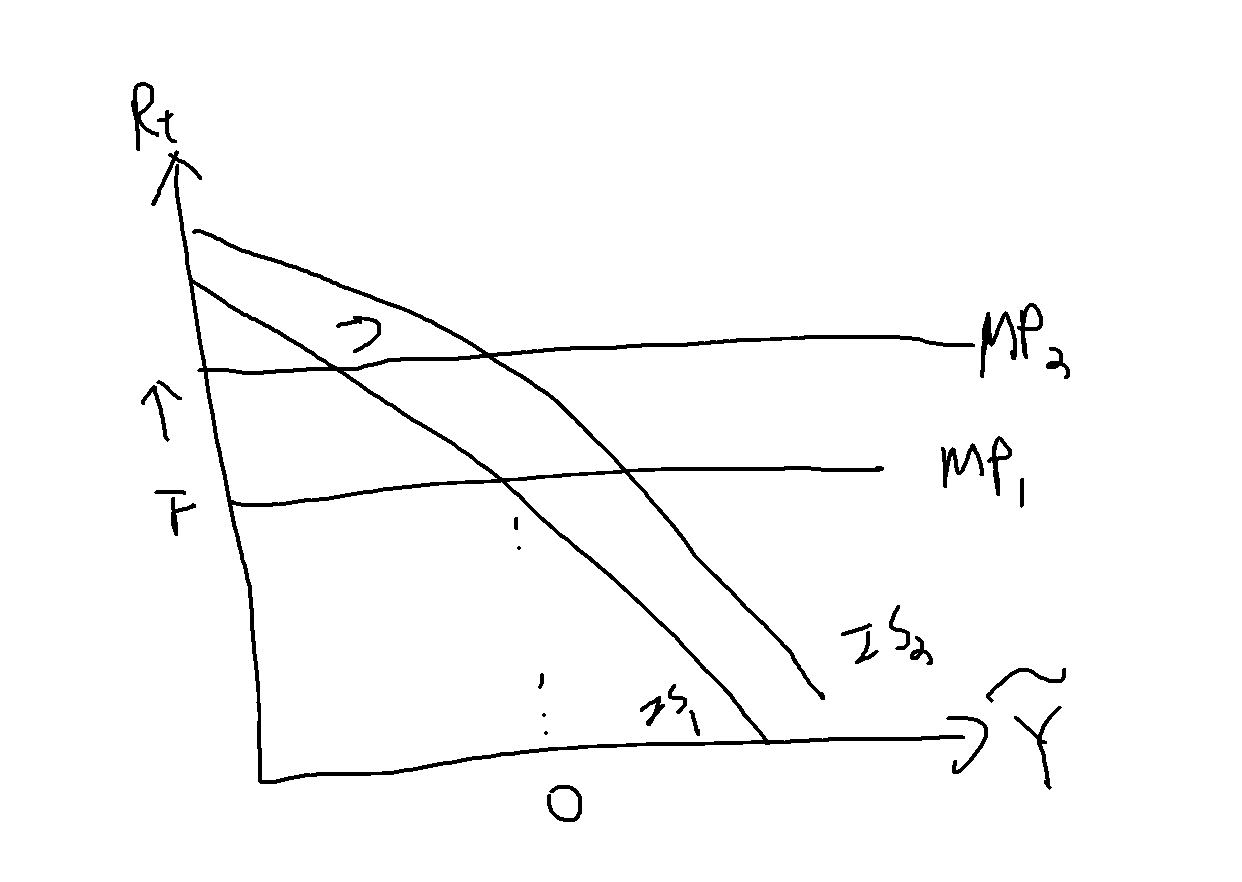
\includegraphics[width=0.5\linewidth]{figure/q4b}
	\end{figure}
	
	\clearpage
	
	\item \textbf{(3 pts)} In the event of a recession, if the government implements a discretionary policy to stimulate the economy, is it necessary for the government to spend more than the decrease in output to bring current output to potential output levels? Please provide the rationale behind your answer in 3-4 sentences.
	\vspace{1cm}
	\item[] \textbf{soln:}  The government does not need to spend more than 10\% to boost the economy back to the potential output level. That's because of the multiplier effect. Each dollar the government spend would be multiplied because there would be sequence increase in investment (dictated by $\bar{x}$).
	\vspace{1cm}
	\item \textbf{(3 pts)} If the parameter $\bar{x}$ increases, how does it affect the effectiveness of monetary policy and the fiscal policy? How should we interpret this increase in the parameter $\bar{x}$? Please provide the rationale behind your answer in 3-4 sentences.
	\vspace{1cm}
	\item[] \textbf{soln:} For the same amount of changes in both monetary and fiscal policy, output would experience a larger changes, making the policies more effective. An increase in $\bar{x}$ indicates that an increase investment due to a rise in short-run output, possibly caused by increased cash flow during an economic boom.
\end{enumerate}

%\newpage
%\begin{center}
%	This page intentionally left blank. Please continue your answer for q.2 below.
%\end{center}
%\vspace*{\fill}

\clearpage
\item  \textbf{(10 pts)}\label{P4} Suppose you have been tasked with analyzing the performance of four different countries. These countries share the same production function, expressed as $Y= \bar{A} N^{1-\alpha} K^{\alpha}$.

\begin{enumerate}[label=(\alph*)]
	
	
	\item \textbf{(2 pts)} Convert the production into the intensive form.
	\vspace{1cm}
	\item[] \textbf{soln:} \[\frac{Y}{N}= \frac{\bar{A} N^{1-\alpha} K^{\alpha}}{N} = \frac{AK^{\alpha}}{N^\alpha} = Ak^\alpha\]
	
	\vspace{1cm}
	\item \textbf{(2 pts)} Below is a sample of various countries with their production parameter value $\alpha$, output per capita $y$, and capital per capita $k$, \textit{all relative to the U.S}. Please fill in the missing cells (column $\bar{A}$).
	
	% Table generated by Excel2LaTeX from sheet 'Sheet1'
	\begin{table}[htbp]
		\centering
		\begin{tabular}{p{7.135em}cccc}
			\multicolumn{1}{l}{} & $\alpha$ & $y$ & $k$ & $\bar{A}$ \\
			\midrule
			Country A & 0.39  & 0.02  & 0.01  &  \\
			Country B & 0.44  & 0.29  & 0.40  &  \\
			Country C & 0.35  & 1.21  & 1.40  &  \\
			Country D & 0.43  & 0.24  & 0.31  &  \\
			\bottomrule
		\end{tabular}%
	\end{table}%
	\textbf{Soln}
		\begin{table}[htbp]
				\centering
				\begin{tabular}{p{7.135em}cccc}
						\multicolumn{1}{l}{} & $\alpha$ & $y$ & $k$ & $\bar{A}$ \\ \hline
						Country A & 0.39  & 0.02  & 0.01  & 0.1205 \\
						Country B & 0.44  & 0.29  & 0.4   & 0.4340 \\
						Country C & 0.35  & 1.21  & 1.4   & 1.0756 \\
						Country D & 0.43  & 0.24  & 0.31  & 0.3971 \\
						\bottomrule
					\end{tabular}%
				\label{tab:addlabel}%
			\end{table}%
	
	
	\newpage
	\item \textbf{(2 pts)}   What can we say about a country if its $\bar{A} = 1$?
	\vspace{1cm}
	\item[] \textbf{soln:} It has a TFP that is the same as the US.
	\vspace{2cm}
	\item \textbf{(2 pts)} What might help explain why $\bar{A} >1$?
	\vspace{1cm}
	\item[] \textbf{soln:} This implies TFP that is higher than the US. It can be because the country has a better human capital. 
	\vspace{2cm}
	\item \textbf{(2 pts)} What might cause the differences in $\alpha$?
	\vspace{1cm}
	\item[] \textbf{soln:}The answer to this lies in differences in capital intensities across countries. Note, generally speaking, developing countries have lower capital shares than developed countries, given the endowments of resources and prices of those resources
	
\end{enumerate}

\newpage

\item  \textbf{(20 pts)}\label{P5} This question relates to the Romer growth model discussed in Chapter 6. Orangeville, a closed economy without government spending, features a production function:

\[Y_t = A_t L_{y,t}\]

Here, \(Y_t\) represents the output, \(L_{y,t}\) stands for the labor employed and $A_t$ stand for TFP (or stock of ideas) in period \(t\). Orangeville's  accumulation of ideas  following:

\[\Delta A_{t+1} = \bar{z}A_t L_{a,t}\]
where $\bar{z}$ is the productivity of idea creation and $L_{a,t}$ is the amount of labour in the idea sector.

The sum of numbers of workers ($L_{y,t}$) and researchers ($L_{a,y}$) equal to the total population: $L_{y,t} + L_{a,t} = \bar{L}$.  The labor supply is inelastic, with the economy consistently providing \(\bar{L}\) units of labor at any given wage. Meanwhile, there are $\ell$ proportion of the population work in the idea production.

\begin{enumerate}[label=(\alph*)]
	\item \textbf{(2 pts)} In one to two sentences, explain what it means economically for the variable $A_t$ to be in both the production function and ideas accumulation function.
	
	\vspace{1cm}
	\item[] \textbf{soln:} Ideas are nonrival which mean many people can benefit from and simultaneously, $A_t$ improve both good and research production.
	\clearpage
	\item \textbf{(5 pts)} 
	Determine the balanced growth path of GDP per capita as a function of exogenous variables and parameters, and interpret the growth rate of GDP per capita.
	\vspace{1cm}
	\item[] \textbf{soln:}
	\[\Delta A_{t+1} = \bar{z} A_t L_{a,t} \implies \frac{\Delta A_{t+1}}{A_t} = g_A = \bar{z} \bar{\ell} \bar{L}\]
	
	\[A_t = A_0 (1+g_A)^t\]
	
	\[Y_t = A_0 (1+g_A)^t L_{y,t} = A_0 (1+g_A)^t (1-\bar{\ell}) \bar{\ell}\]
	
	\[y_t = \frac{Y_t}{\bar{L}} = A_0 (1+g_A)^t (1-\bar{\ell})\]
	
	The growth rate of GDP per capita is a function of productivity in the research sector, $\bar{z}$ and the fraction of researcher (1-$\bar{\ell}$)
	\clearpage
	\item \textbf{(8 pts)} 	Consider the scenario where the economy encounters a large influx of foreign laborers, denoted as $L_r$, who are not skilled in work in the research sector and thus can only contribute to the goods production sector. 
	\begin{enumerate}
		\item Compute the short run output per capita. Compare it with the output per capita before and after these foreign laborers arrive. 
		\vspace{1cm}
		\item[] \textbf{soln:} The labour supply in the production sector become:
		\[L_{y,t} = (1-\bar{\ell}) \bar{L} + L_r\]
		
		\[Y_t = A_t \left((1-\bar{\ell}) \bar{L} + L_r\right)\]
		
		\[y_t = \frac{Y_t}{\bar{L} + L_r} = A_0 (1+g_A)^t \left[\frac{(1-\bar{\ell}) \bar{L} + L_r}{\bar{L} + L_r}\right]\]
		
		The $y_t$ has increase after the influx of foreign labour.
		
		\[\frac{(1-\bar{\ell}) \bar{L} + L_r}{\bar{L} + L_r} > 1-\bar{\ell}\]
		
		\[(1-\bar{\ell}) \bar{L} + L_r > (1-\bar{\ell}) (\bar{L} + L_r)\]
		
		\[L_r > (1-\bar{\ell}) L_r\]
		
		\item Why is it higher or lower compare to before these foreign laborers arrive?
		\vspace{1cm}
		\item[] \textbf{soln:} That is because there are more workers in the production sector (proportionally).
		
		\item What would happen to the long-run growth rate?
		\vspace{1cm}
		\item[] \textbf{soln:} It would be unchanged as none of these worker work in the research sector.
		
		\item Draw a ratio-scale graph to depict how this change affects the current level and future growth path of GDP per capita. Assuming these foreigner would not switch to research sector at any time in the future.
		\vspace{1cm}
		\item[] \textbf{soln:}
		
		\begin{figure}[htbp!]
			\centering
			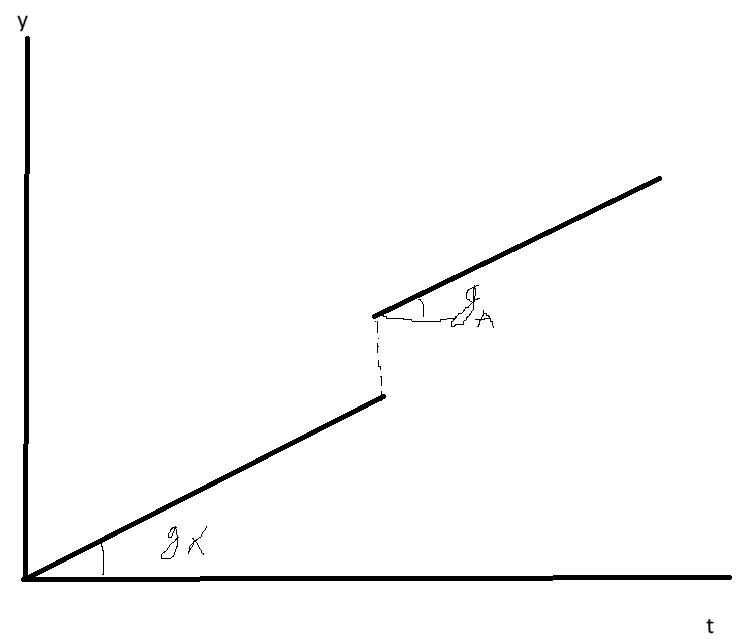
\includegraphics[width=0.7\linewidth]{figure/soln1}
		\end{figure}
		
		
	\end{enumerate}
%	\newpage
%	\begin{center}
%		This page intentionally left blank. Please continue your answer below.
%	\end{center}
%	\vspace*{\fill}
	\clearpage
	\item \textbf{(5 pts)} 	What would be the effect on the initial impact on GDP per capita and the long-run growth rate if all foreign laborers, instead of being limited to the production sector, they have high research skills and would all join the research sector? Explain and illustrate this change using a ratio-scale graph, showing both the current level and future trajectory of GDP per capita (you do not need to compute the equation like in part c.i).
	\vspace{1cm}
	\item[] \textbf{soln:}
	
	\begin{figure}[htbp!]
		\centering
		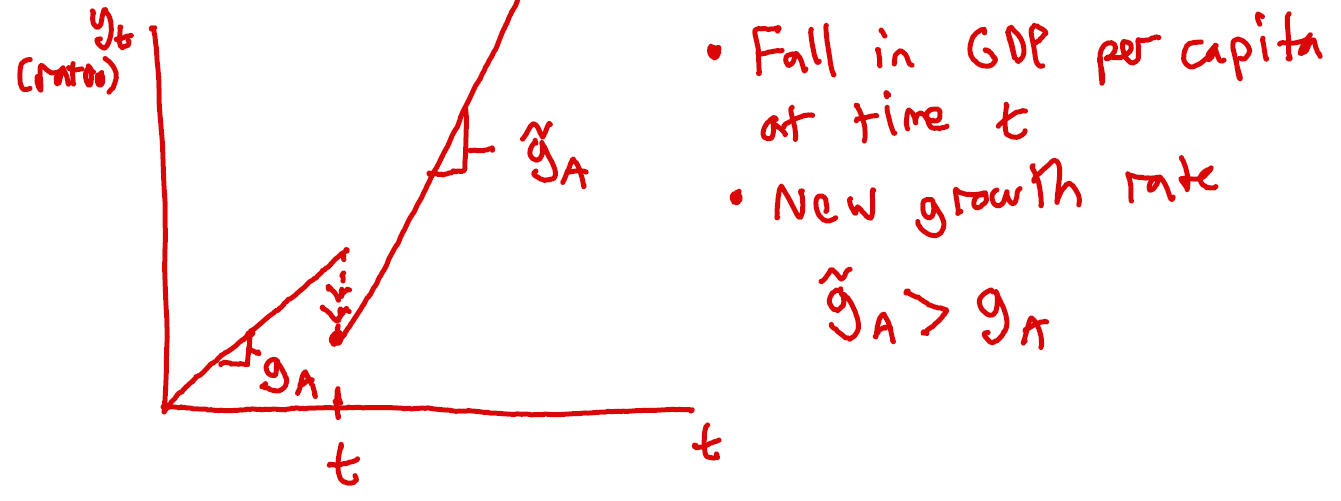
\includegraphics[width=0.9\linewidth]{figure/soln2}
	\end{figure}
	
	
\end{enumerate}

%\newpage
%\begin{center}
%	This page intentionally left blank. Please continue your answer below.
%\end{center}
%\vspace*{\fill}
%
%\newpage
%\begin{center}
%	This page intentionally left blank. Please continue your answer below.
%\end{center}
%\vspace*{\fill}

\newpage

\item  \textbf{(10 pts)}\label{P6} 
There are two countries, country A and country B. Both countries have the same production function: $Y=\bar{A} N^{1/2} K^{1/2}$. Country A is experiencing a growth rate of 3\% per year. Meanwhile, in country B, we know the growth rate of capital ($K$) is 2\% and the total factor productivity (TFP) growth is 1\%. Labor is not growing in either country. In the year 2000, the GDP per capita of country A is \$10,000, and the GDP per capita of country B is \$28,000. With the assistance of foreign investment and technology diffusion, country A can achieve a growth rate of 5\% in the initial 20 years.


\begin{enumerate}[label=(\alph*)]
	\item \textbf{(2 pts)} Express the growth rate of output per capita using the production function. Then, calculate country B's growth rate.
	\vspace{1cm}
	\item[] \textbf{soln:} \[g_Y = g_A + 0.5 g_N + 0.5 g_K\]
			\[g_y = g_A  + 0.5 g_k\]
			\[g_{y,B} = 1\% + 0.5(2\%) = 2\%\]
	\vspace{1cm}
	\item \textbf{(3 pts)} How long would it take for country A to catch up with country B? 
	\vspace{1cm}
	\item[] \textbf{soln:} 
	\[10000 (1.05)^{20}(1.03)^{t-20} = 28000 (1.02)^t\]
	\[\frac{(1.03)^{t}}{(1.03)^{20}(1.02)^t} = \frac{28000}{10000 (1.05)^{20}} \to \left(\frac{1.03}{1.02}\right)^t = \frac{28000(1.03)^{20}}{10000 (1.05)^{20}} \]
	\[t \ln\left(\left(\frac{1.03}{1.02}\right)\right) = \ln\left(\frac{28000(1.03)^{20}}{10000 (1.05)^{20}} \right)\]
	\[t = 66.111\]
	
	\clearpage
	\item \textbf{(3 pts)} Draw a ratio scale graph with GDP per capita on the y-axis and year on the x-axis to illustrate the case in part b). Clearly label all the axis and important points of interest.
	\vspace{1cm}
	\item[] \textbf{soln:} 
	\begin{figure}[htbp!]
		\centering
		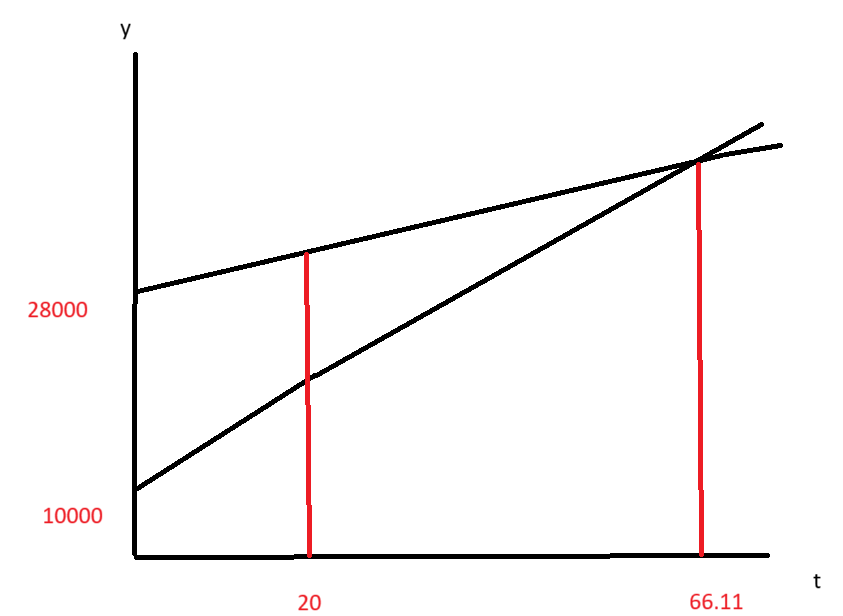
\includegraphics[width=0.7\linewidth]{figure/soln3}
	\end{figure}
	
	
	\clearpage
	\item \textbf{(2 pts)} List two points each regarding the benefits and costs of growth.
	\vspace{1cm}
	\item[] \textbf{soln:} 
	
	Benefit: Improvements in health, Higher incomes, Increase in the variety of goods and services
	
	Cost: Environmental problems, Income inequality across and within countries, Loss of certain types of jobs
	
\end{enumerate}


\newpage
\begin{center}
	This page intentionally left blank. Please continue your answer below.
\end{center}
\vspace*{\fill}
%
%\newpage
%\begin{center}
%	This page intentionally left blank. Please continue your answer below.
%\end{center}
\vspace*{\fill}

\centering{-- The End -- }
\end{enumerate}
  \end{document}
